% source: https://git.fslab.de/mmklab/latex-templates/tree/master/presentation

\documentclass{beamer}

%\useoutertheme{progress}

\usepackage{etoolbox}
\newtoggle{german}

% % % % % LANGUAGE % % % %
% Make your choice here
\togglefalse{german} % English
%\toggletrue{german} % German
% % % % % \LANGUAGE % % % %

% % % Handouts % % %
%\usepackage{handoutWithNotes}
%\pgfpagesuselayout{2 on 1 with notes landscape}[a4paper,border shrink=5mm]
% % % Handouts % % %


\iftoggle{german}{
\usepackage[ngerman]{babel} % Deutsche Sprachanpassungen
\usepackage[T1]{fontenc}    % Silbentrennung bei Sonderzeichen
\usepackage[utf8]{inputenc} % Direkte Angabe von Umlauten im Dokument.Wenn Sie an einem Mac sitzen,verwenden Sie ggf. „macce“ anstatt „utf8“.
\usepackage[autostyle=true,german=quotes]{csquotes} % Anfuehrungszeichen\
}{
\usepackage[utf8]{inputenc}}


\usepackage[utf8]{inputenc}
\usepackage[T1]{fontenc}
\usepackage{textcomp}
\setbeamercovered{transparent}
\usepackage{default}
\usepackage{lmodern}
\usepackage{amsmath,amsfonts,amssymb} % Mathe
\usepackage{eurosym}
\usepackage{tikz}
\usepackage{graphicx}
\usepackage[labelformat=empty]{caption}
\usepackage{verbatim}
\usepackage{color}
\usepackage{hypernat}
\usepackage{tabularx}
\usepackage[]{units}
\usepackage{caption}
\usepackage{comment}
%\usepackage{subfigure}
\usepackage{wasysym}
\usepackage{ulem}
\usepackage[printonlyused]{acronym} 
\usepackage{tabularx}
\usepackage{appendixnumberbeamer}
\usepackage{epigraph}
\usepackage{remreset}% tiny package containing just the \@removefromreset command
\usepackage{subcaption}
\usepackage{pdfpcnotes}% Usefull package for notes for presentations
\usepackage{colorbar}
%\usepackage{./progbar}
%\usepackage{./beamerouterthemeprogress}

\let\Tiny=\tiny % Reduces a few recent error on Unix systems

\usepackage[sorting=none,style=numeric-comp,backend=bibtex,firstinits=true]{biblatex} % load the package
\addbibresource{./references.bib} % Add your bib file
\renewcommand*{\bibfont}{\footnotesize}

% % % % Style % % % %
% Some colours as used in other programms like openoffice
\definecolor{red}{RGB}{184,71,71}
\definecolor{green}{RGB}{51,204,102}
\definecolor{blue}{RGB}{0,153,255}
\definecolor{fhblau}{rgb}{0, 0.594, 0.949}

\setbeamercolor{title}{bg=fhblau, fg=white}
\setbeamercolor{frametitle}{bg=fhblau, fg=white}
\setbeamercolor{structure}{fg=fhblau}

% MISC Styles %
\setbeamertemplate{bibliography item}[text]
\usetheme{default}
\setbeamertemplate{footline}[frame number]
\setbeamersize{text margin left=0.3cm,text margin right=0.3cm}
\setbeamertemplate{navigation symbols}{}%remove navigation symbols
\makeatletter
\@removefromreset{subsection}{section}
\makeatother
\setcounter{subsection}{1}


% Here are some usefulf different fonts. Use them in every flooting enviroment with \usebeamerfont{AAA}
\setbeamerfont{AAA}{size*={16.00}{15.00}}
\setbeamerfont{aaa}{size*={12.00}{11.00}}
\setbeamerfont{bbb}{size*={11.00}{11.00}}
\setbeamerfont{ccc}{size*={10.00}{11.00}}
\setbeamerfont{ddd}{size*={9.00}{11.00}}
\setbeamerfont{eee}{size*={8.00}{11.00}}
\setbeamerfont{fff}{size*={7.75}{10.75}}
\setbeamerfont{ggg}{size*={7.50}{10.50}}
\setbeamerfont{hhh}{size*={7.25}{10.25}}
\setbeamerfont{iii}{size*={7.00}{10.00}}
\setbeamerfont{jjj}{size*={6.00}{9.00}}
\setbeamerfont{kkk}{size*={5.00}{8.00}}
\setbeamerfont{lll}{size*={4.00}{7.00}}
\setbeamerfont{mmm}{size*={3.00}{6.00}}
\setbeamerfont{nnn}{size*={2.00}{5.00}} 

% Set some beamer fonts
\setbeamerfont{title}{size=\Large,series=\bfseries,parent=structure}
\setbeamerfont{caption}{size=\footnotesize \itshape}
\setbeamertemplate{footline}[text line]{%
	\parbox{\linewidth}{\vspace*{-8pt}\hspace{1em}\insertshortauthor\hspace{8mm} Sematic Segmentation using Resource Efficient Deep Learning \hfill\insertpagenumber/\inserttotalframenumber}}

\renewcommand*{\bibfont}{\usebeamerfont{kkk}}

% A new cell type
\newcommand{\specialcell}[2][c]{%
  \begin{tabular}[#1]{@{}c@{}}#2\end{tabular}}

% This is usefull if you want to use enumerations over several frames
\newcounter{saveenumi}
\newcommand{\seti}{\setcounter{saveenumi}{\value{enumi}}}
\newcommand{\conti}{\setcounter{enumi}{\value{saveenumi}}}

% logo of my university
\titlegraphic{
\centering %
\includegraphics[height=1.5cm]{./logos/logo_hbrs.png} \hspace{2cm} % For external companies

\includegraphics[height=1.5cm]{./logos/logo_hbrs.png}}


% % % % % Opening % % % %
\title[]{Sematic Segmentation using\\ Resource Efficient Deep Learning}
\author[Naresh Kumar Gurulingan]{Naresh Kumar Gurulingan \\ \footnotesize naresh.gurulingan@smail.inf.h-brs.de}
\date{\today}
\institute[HBRS]{Hochschule Bonn-Rhein-Sieg}
\def\ThesisPubDate{\today} % Change here to the date you are going to print your thesis
\subject{Sematic Segmentation using Resource Efficient Deep Learning}
\keywords{}


\begin{document}

% Title Frame
\begin{frame}
\pnote{Here are some nodes. They are not visible on the first slides} % Notes
\titlepage
\end{frame}

\iftoggle{german}{
\begin{frame}{Agenda}
\usebeamerfont{ccc}
\tableofcontents
\end{frame}
}{
\begin{frame}{Table of Contents}
\usebeamerfont{ccc}
\tableofcontents
\end{frame}
}

\section{Introduction}
% First Frame
\begin{frame}{Introduction}

	\textbf{Semantic segmentation}
	
	Divide an input image into different regions which contain a desired object or background.
	
	\begin{figure}[!htb]
		\centering
		
\includegraphics[width=.6\linewidth]{images/em_01_023}
		\caption{Left: Input image; Right: Segmentation result.}
		\label{Fig:real}
	\end{figure}

\end{frame}

\section{Applications}
% First Frame
\begin{frame}{Applications}
	\begin{itemize}
  \item[a] {
    Autonomous cars
  }
  \item[b] {
    Robotics
  }
  \item[c] {
    Augmented reality
  }
  \end{itemize}
  
  \begin{figure}
		\begin{subfigure}{0.3\textwidth}
			\centering
			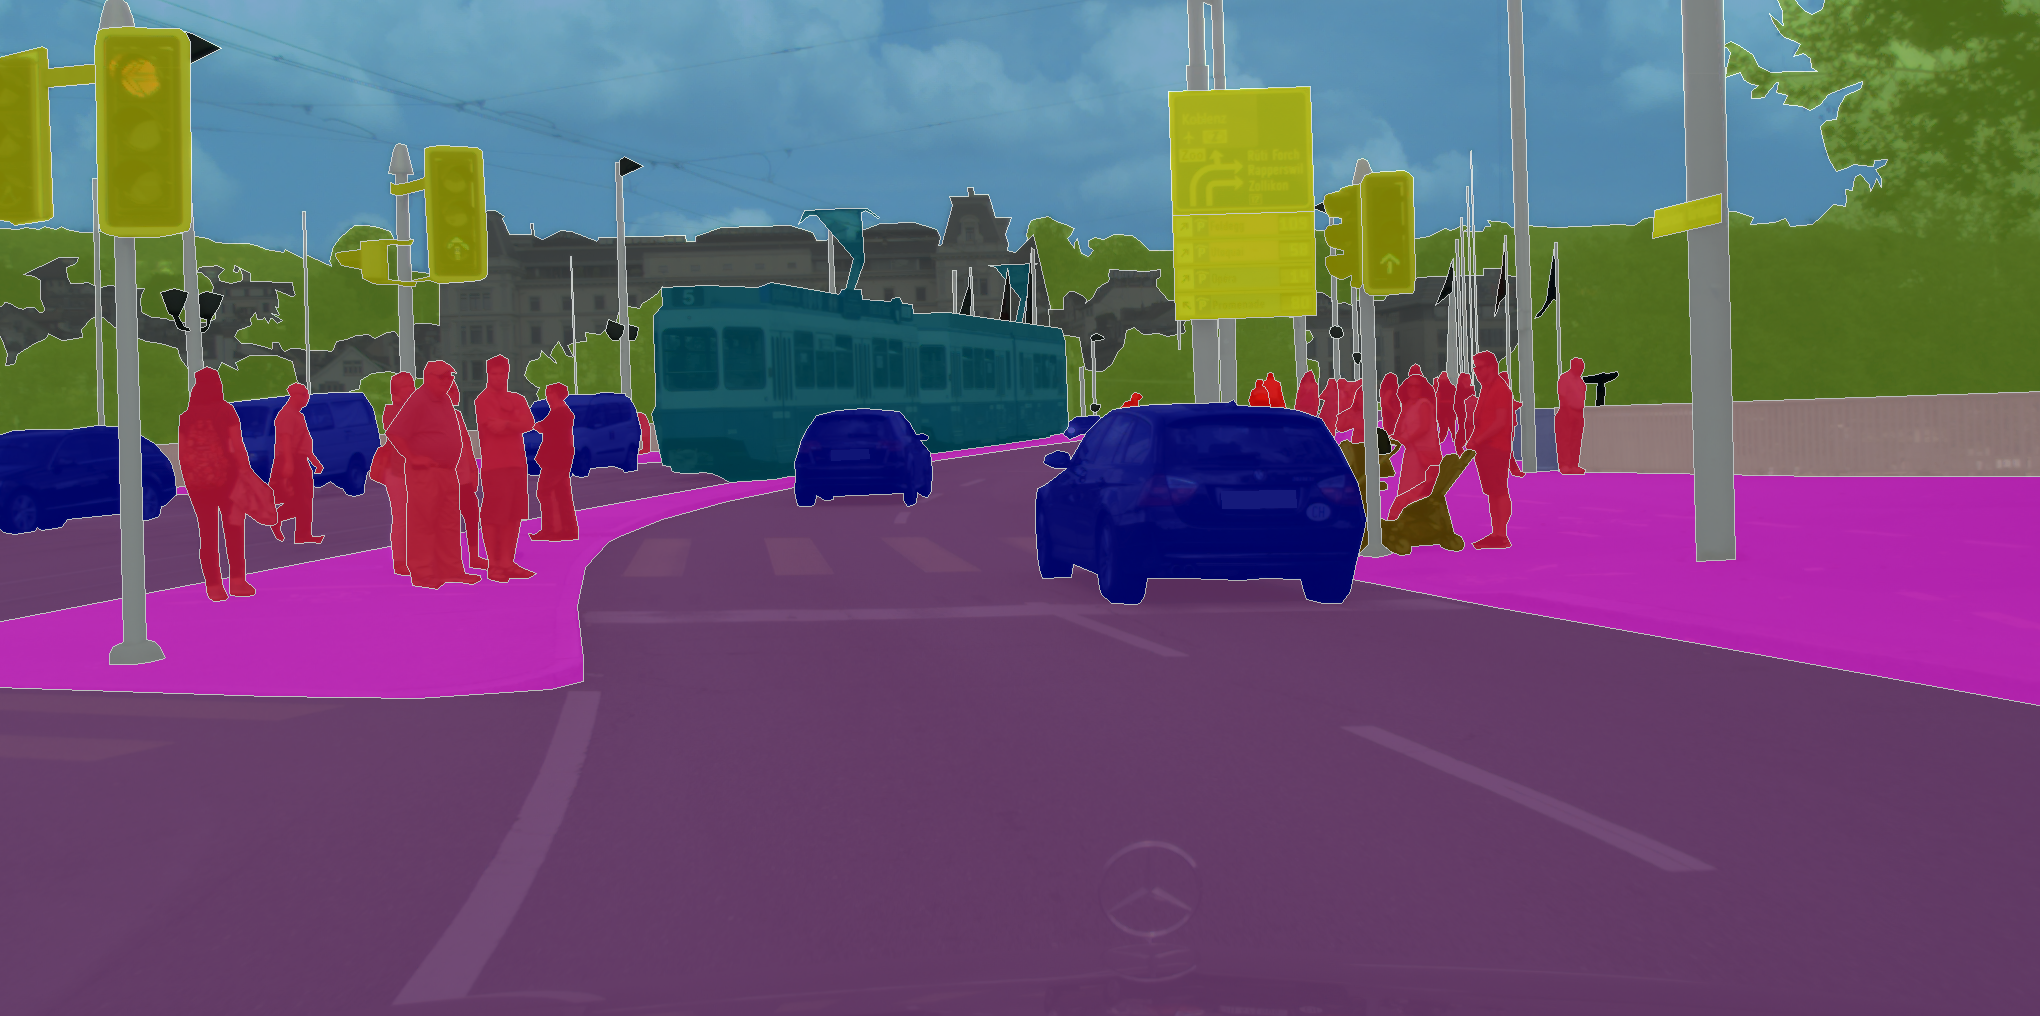
\includegraphics[width=0.95\linewidth]{images/auto_driving}
			\caption{Street scene}
		\end{subfigure}
		\begin{subfigure}{0.3\textwidth}
			\centering
			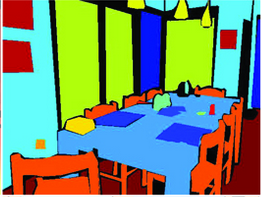
\includegraphics[width=0.8\linewidth]{images/indoor}
			\caption{Indoor scene}
		\end{subfigure}
		\begin{subfigure}{0.3\textwidth}
			\centering
			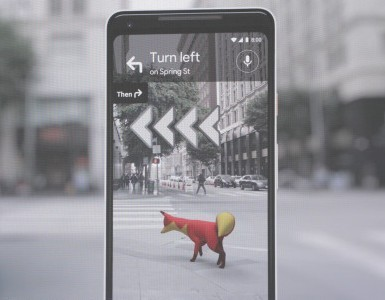
\includegraphics[width=0.8\linewidth]{images/vr_dog}
			\caption{Augmented guide}
		\end{subfigure}
		%\caption{(a)Street scene, (b) Indoor scene, (c) Augmented guide.}
		\label{Fig:app}
	\end{figure}

\end{frame}

\section{Dataset}

\begin{frame}{Dataset}
	
	\textbf{Objects in the dataset}
	\begin{figure}[h]
		\centering
		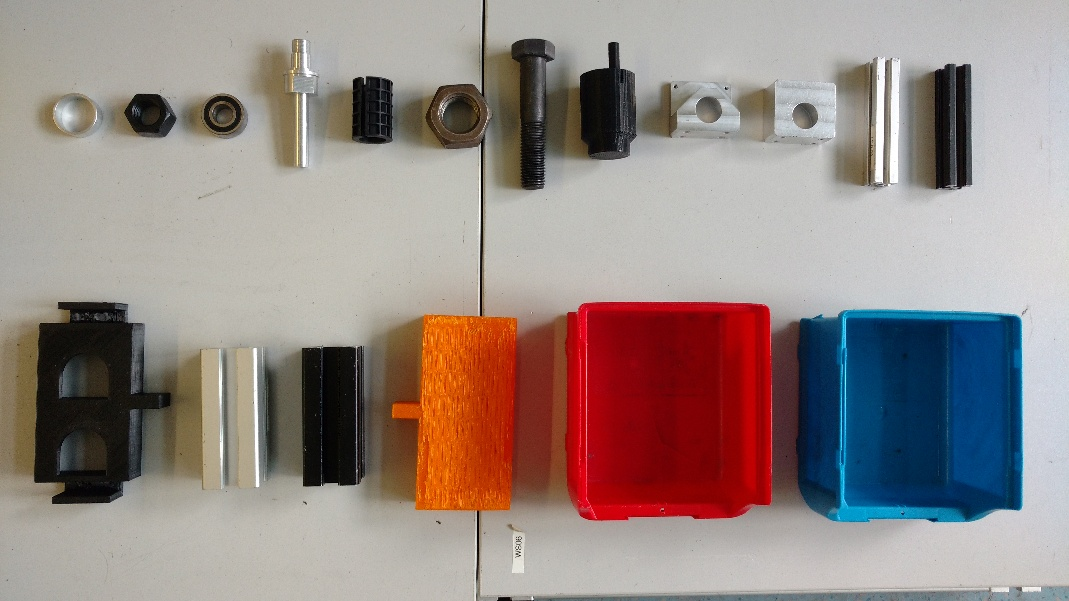
\includegraphics[scale=0.2]{images/all_objects}
		\caption{This figure shows all the 18 objects in the dataset. First row from left: "distance\_tube", "m20", "bearing", "axis", "r20", "m30", "m20\_100", "motor", "bearing\_box\_ax16", 'bearing\_box\_ax01", "f20\_20\_B", "f20\_20\_G". Second row from left: "em\_01", "s40\_40\_B", "s40\_40\_G", "em\_02", "container\_box\_red", "container\_box\_blue".}
		\label{Fig:allobjects}
	\end{figure}

\end{frame}

\section{Annotation process}

\begin{frame}{Annotation process}


\end{frame}

\section{Artificial image generation}

\begin{frame}{Artificial image generation}


\end{frame}

\section{Dataset variants}

\begin{frame}{Dataset variants}


\end{frame}

\section{Dataset analysis}

\begin{frame}{Dataset analysis}


\end{frame}

\section{DeepLabv3+}

\begin{frame}{DeepLabv3+}


\end{frame}


\begin{frame}{DeepLabv3+}


\end{frame}

\begin{frame}{DeepLabv3+}


\end{frame}

\section{Results}

\begin{frame}{Results}


\end{frame}


\begin{frame}{Results}


\end{frame}


\begin{frame}{Results}


\end{frame}


\begin{frame}{Results}


\end{frame}

\begin{frame}{Results}


\end{frame}


\begin{frame}{Results}


\end{frame}


\begin{frame}{Results}


\end{frame}


\begin{frame}{Results}


\end{frame}


\begin{frame}{Results}


\end{frame}


\begin{frame}{Results}


\end{frame}

\section{Contributions and future work}

\begin{frame}{Conclusion and future work}
\textbf{Contributions}
	\begin{itemize}
		\item Artificial image generation algorithm.
		\item Segmentation dataset with 18 atWork objects.
		\item Evaluation of DeepLabv3+ with resource efficient encoders MobileNetv2 and Xception.
	\end{itemize}
	
\vspace{5mm}
\textbf{Future work}
	\begin{itemize}
		\item Model interpretability.
		\item Architecture search.
		\item Fusion of 2D image data with point cloud information.
	\end{itemize}

\end{frame}


\begin{frame}{Thank you very much!}
\usebeamerfont{AAA}
Are there any questions? \\
\end{frame}

\begin{frame}
  \frametitle{References}
  \printbibliography[title={References}]   
\end{frame}

\end{document}
